\documentclass{article}

\usepackage{listings}
\usepackage{pgfplots}

\begin{document}
The objective was to find optimal tile sizes for the matrix multiplication, the tile sizes for dimension x and y were allowed to be different.

The matrix size is 128x128 and the number of workers range from 1 to 18. This time the multiplication C = A * B was performed with matrix A in row format and matrix B in column format (better cache utilization) - in contrast to the tests of the last week. SBX was used for the crossover, ``parameter based mutation'' was used as mutation operator.

128x128: For each parameter setting, the test was repeated 50 times to get more confidence in the results, 900 tests were performed (50 * 18):
\begin{itemize}
  \item 50 tests per setting
  \item 18 different worker sizes (from 1 to 18)
\end{itemize}

1000\_50\_256x256: For each parameter setting, the test was repeated 50 times to get more confidence in the results, 900 tests were performed (50 * 18):
\begin{itemize}
  \item 50 tests per setting
  \item 18 different worker sizes (from 1 to 18)
\end{itemize}

1000\_100\_256x256 and more: For each parameter setting, the test was repeated 5 times to get more confidence in the results, 90 tests were performed (5 * 18):
\begin{itemize}
  \item 50 tests per setting
  \item 18 different worker sizes (from 1 to 18)
\end{itemize}

% \section{Population 50}
\begin{figure}[h]
  \centering
  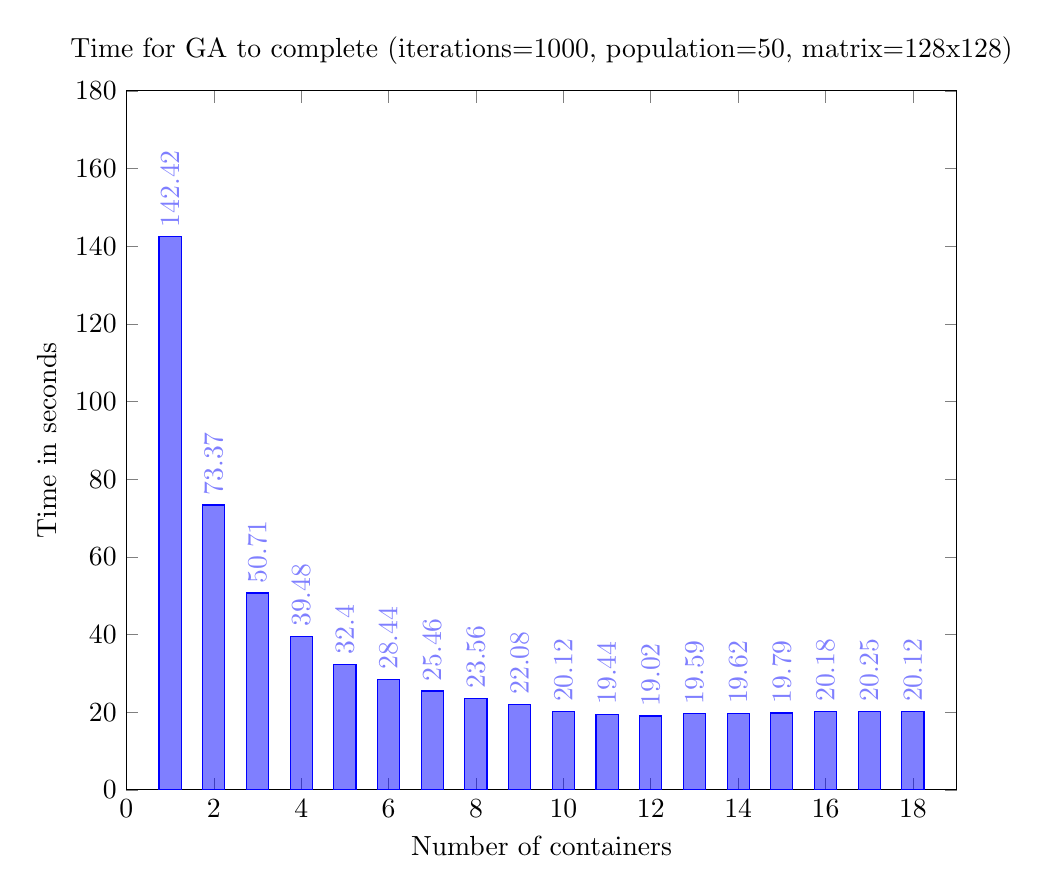
\begin{tikzpicture}[]
    \begin{axis}[
	title={Time for GA to complete (iterations=1000, population=50, matrix=128x128)},
	xlabel={Number of containers},
	ylabel={Time in seconds},
	width=\linewidth,
	enlargelimits=false,
	nodes near coords=\rotatebox{90}{\pgfmathprintnumber[]\value},
	visualization depends on=rawy \as \value,
	xmin=0,
	xmax=19,
	ymin=0,
	ymax=180
      ]
      \addplot[ybar, bar width=8pt, blue, fill, fill opacity=0.5]
      coordinates{(1,142.41692) (2,73.3701) (3,50.7134) (4,39.47686) (5,32.40048) (6,28.43836) (7,25.45766) (8,23.5593) (9,22.08228) (10,20.12404) (11,19.44024) (12,19.02386) (13,19.59172) (14,19.61892) (15,19.79174) (16,20.17862) (17,20.25264) (18,20.12062)};
%       \addplot [red, no markers] coordinates {(0,0) (12,38.4)};
    \end{axis}
  \end{tikzpicture}
  \caption{Find an optimal tile size for the tiled matrix multiplication. The x-axis shows the number of containers (workers), the y-axis shows the time it took to finish. iterations=1000, population=50, matrix size=128x128}
\label{plot:tiledmul_1000_50_128x128}
\end{figure}

\begin{figure}[h]
  \centering
  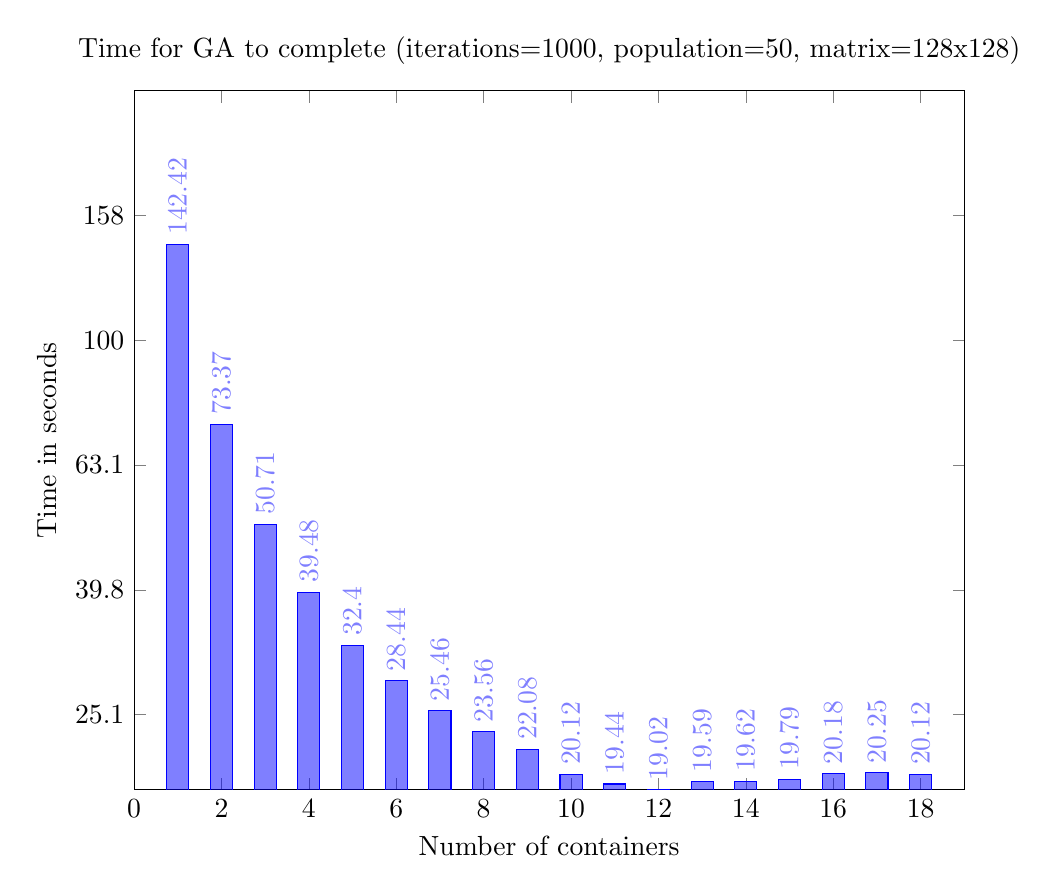
\begin{tikzpicture}[]
    \begin{semilogyaxis}[
	title={Time for GA to complete (iterations=1000, population=50, matrix=128x128)},
	xlabel={Number of containers},
	ylabel={Time in seconds},
	width=\linewidth,
	enlargelimits=false,
% 	nodes near coords,
	log ticks with fixed point,
	nodes near coords=\rotatebox{90}{\pgfmathprintnumber[]\value},
	visualization depends on=rawy \as \value,
	xmin=0,
	xmax=19,
	ymin=0,
	ymax=251
      ]
      \addplot[ybar, bar width=8pt, blue, fill, fill opacity=0.5]
      coordinates{(1,142.41692) (2,73.3701) (3,50.7134) (4,39.47686) (5,32.40048) (6,28.43836) (7,25.45766) (8,23.5593) (9,22.08228) (10,20.12404) (11,19.44024) (12,19.02386) (13,19.59172) (14,19.61892) (15,19.79174) (16,20.17862) (17,20.25264) (18,20.12062)};
    \end{semilogyaxis}
  \end{tikzpicture}
  \caption{Find an optimal tile size for the tiled matrix multiplication. The x-axis shows the number of containers (workers), the y-axis shows the time it took to finish on a logarithmic scale. iterations=1000, population=50, matrix size=128x128}
  \label{plot:tiledmul_1000_50_128x128_log}
\end{figure}

\begin{table}
  \centering
  \begin{tabular}{l|r|r}
    & x & y \\ \hline
    min & 69 & 6 \\
    max & 128 & 122 \\
    mean & 126.557268722 & 19.3248898678 \\
    var & 62.330420734 & 94.5651514196 \\
    stddev & 7.894961731 & 9.72446149767 \\
  \end{tabular}
  \caption{Results for tile sizes, iterations=1000, population=50, matrix size=128x128}
  \label{table:tiledmul_1000_50_128x128}
\end{table}

% \section{Population 100}
\begin{figure}[h]
  \centering
  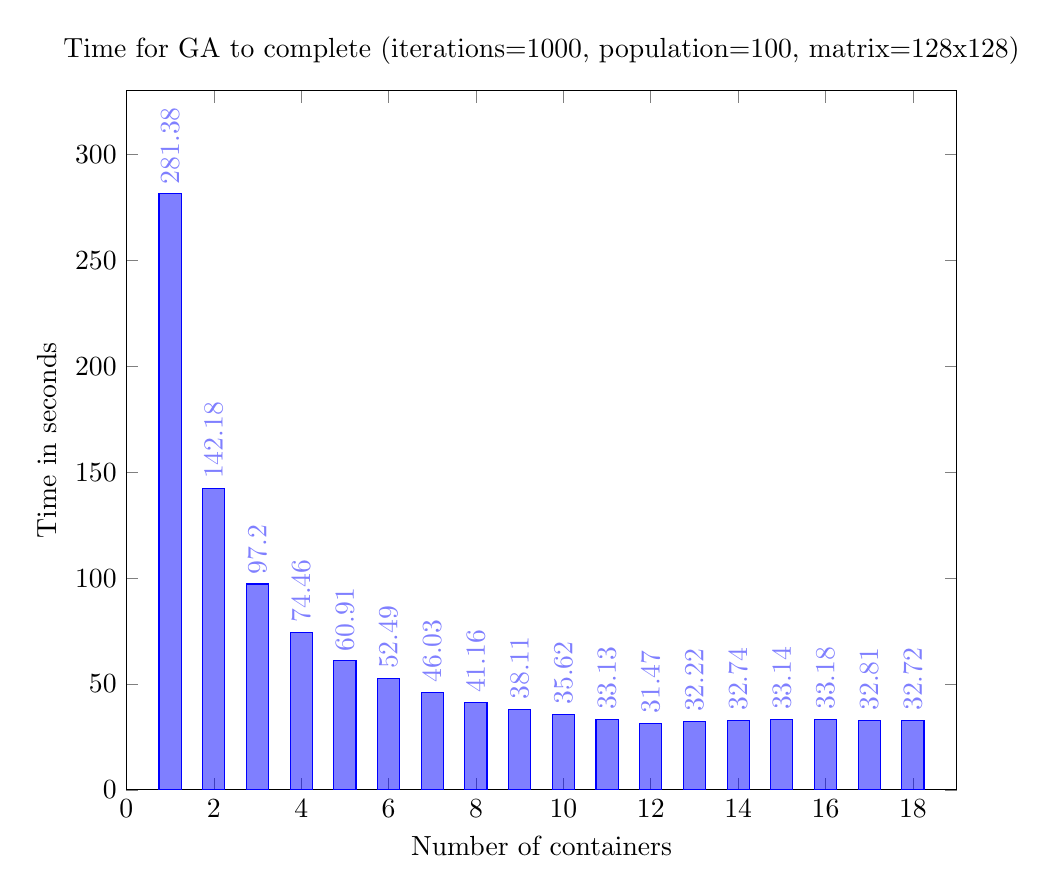
\begin{tikzpicture}[]
    \begin{axis}[
	title={Time for GA to complete (iterations=1000, population=100, matrix=128x128)},
	xlabel={Number of containers},
	ylabel={Time in seconds},
	width=\linewidth,
	enlargelimits=false,
	nodes near coords=\rotatebox{90}{\pgfmathprintnumber[]\value},
	visualization depends on=rawy \as \value,
	xmin=0,
	xmax=19,
	ymin=0,
	ymax=330
      ]
      \addplot[ybar, bar width=8pt, blue, fill, fill opacity=0.5]
      coordinates{(1,281.384215686) (2,142.179519231) (3,97.2028039216) (4,74.45642) (5,60.91278) (6,52.49378) (7,46.03182) (8,41.16142) (9,38.10728) (10,35.62182) (11,33.12934) (12,31.4689) (13,32.2214) (14,32.73556) (15,33.13768) (16,33.1849) (17,32.80716) (18,32.72124)};
%       \addplot [red, no markers] coordinates {(0,0) (12,38.4)};
    \end{axis}
  \end{tikzpicture}
  \caption{Find an optimal tile size for the tiled matrix multiplication. The x-axis shows the number of containers (workers), the y-axis shows the time it took to finish. iterations=1000, population=100, matrix size=128x128}
\label{plot:tiledmul_1000_100_128x128}
\end{figure}

\begin{figure}[h]
  \centering
  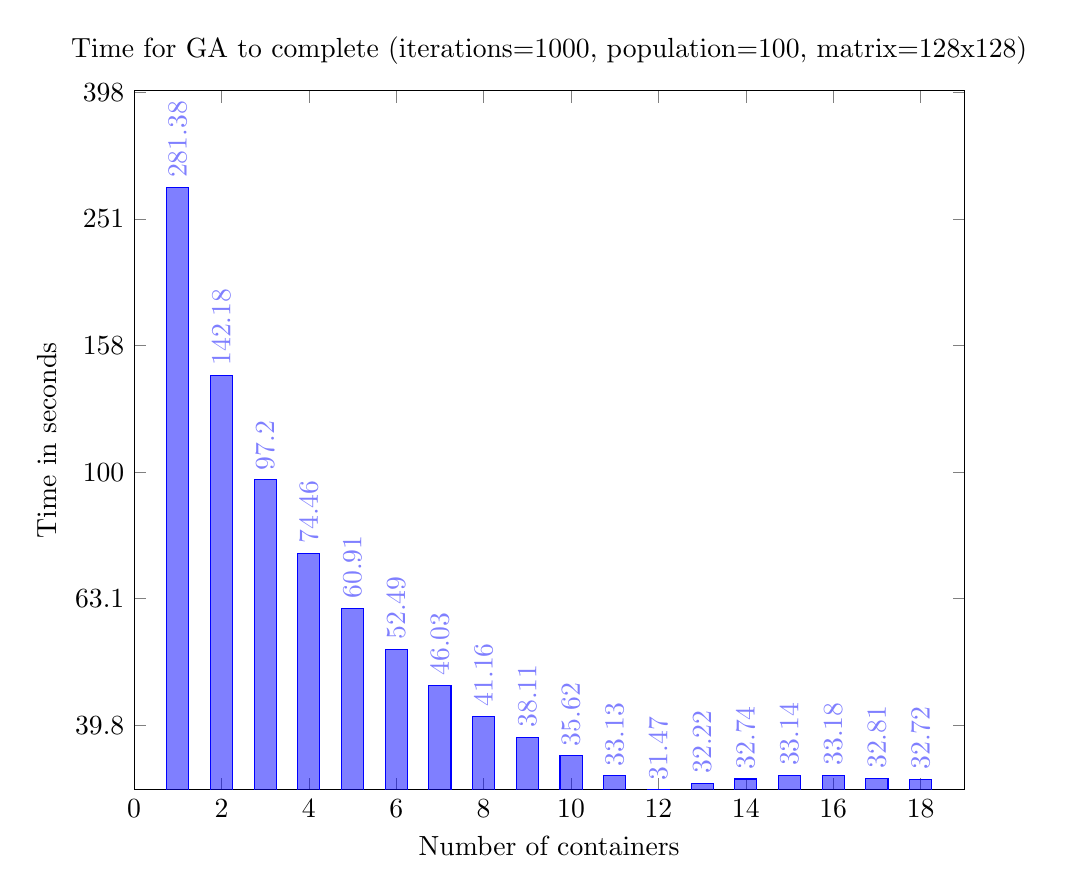
\begin{tikzpicture}[]
    \begin{semilogyaxis}[
	title={Time for GA to complete (iterations=1000, population=100, matrix=128x128)},
	xlabel={Number of containers},
	ylabel={Time in seconds},
	width=\linewidth,
	enlargelimits=false,
% 	nodes near coords,
	log ticks with fixed point,
	nodes near coords=\rotatebox{90}{\pgfmathprintnumber[]\value},
	visualization depends on=rawy \as \value,
	xmin=0,
	xmax=19,
	ymin=0,
	ymax=400
      ]
      \addplot[ybar, bar width=8pt, blue, fill, fill opacity=0.5]
      coordinates{(1,281.384215686) (2,142.179519231) (3,97.2028039216) (4,74.45642) (5,60.91278) (6,52.49378) (7,46.03182) (8,41.16142) (9,38.10728) (10,35.62182) (11,33.12934) (12,31.4689) (13,32.2214) (14,32.73556) (15,33.13768) (16,33.1849) (17,32.80716) (18,32.72124)};
    \end{semilogyaxis}
  \end{tikzpicture}
  \caption{Find an optimal tile size for the tiled matrix multiplication. The x-axis shows the number of containers (workers), the y-axis shows the time it took to finish on a logarithmic scale. iterations=1000, population=100, matrix size=128x128}
  \label{plot:tiledmul_1000_100_128x128_log}
\end{figure}

\begin{table}
  \centering
  \begin{tabular}{l|r|r}
    & x & y \\ \hline
    min & 128 & 5 \\
    max & 128 & 128 \\
    mean & 128.0 & 19.4601769912 \\
    var & 0.0 & 121.854608818 \\
    stddev & 0.0 & 11.0387775056 \\
  \end{tabular}
  \caption{Results for tile sizes, iterations=1000, population=100, matrix size=128x128}
  \label{table:tiledmul_1000_100_128x128}
\end{table}

% \section{Population 200}
\begin{figure}[h]
  \centering
  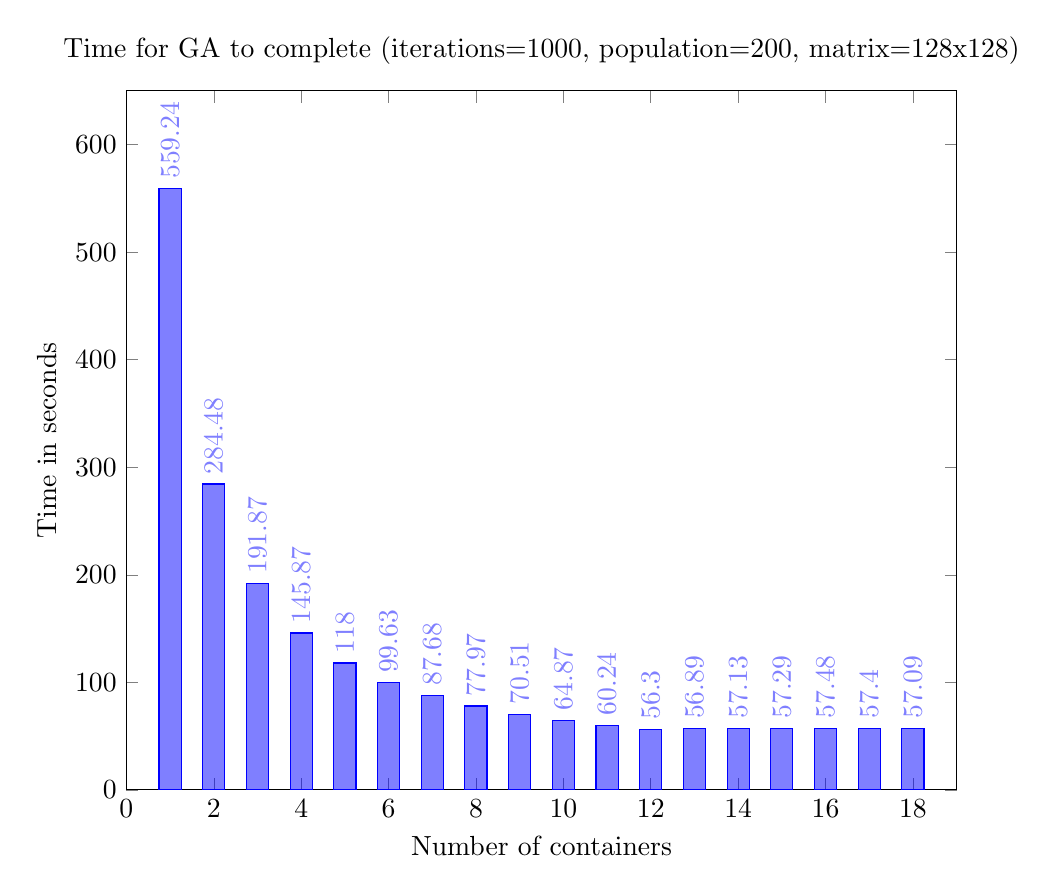
\begin{tikzpicture}[]
    \begin{axis}[
	title={Time for GA to complete (iterations=1000, population=200, matrix=128x128)},
	xlabel={Number of containers},
	ylabel={Time in seconds},
	width=\linewidth,
	enlargelimits=false,
	nodes near coords=\rotatebox{90}{\pgfmathprintnumber[]\value},
	visualization depends on=rawy \as \value,
	xmin=0,
	xmax=19,
	ymin=0,
	ymax=650
      ]
      \addplot[ybar, bar width=8pt, blue, fill, fill opacity=0.5]
      coordinates{(1,559.241803922) (2,284.478117647) (3,191.86994) (4,145.866961538) (5,117.99764) (6,99.62942) (7,87.68198) (8,77.97484) (9,70.50712) (10,64.87274) (11,60.23614) (12,56.29868) (13,56.88716) (14,57.1284) (15,57.29426) (16,57.4755490196) (17,57.4018) (18,57.08912)};
%       \addplot [red, no markers] coordinates {(0,0) (12,38.4)};
    \end{axis}
  \end{tikzpicture}
  \caption{Find an optimal tile size for the tiled matrix multiplication. The x-axis shows the number of containers (workers), the y-axis shows the time it took to finish. iterations=1000, population=200, matrix size=128x128}
\label{plot:tiledmul_1000_200_128x128}
\end{figure}

\begin{figure}[h]
  \centering
  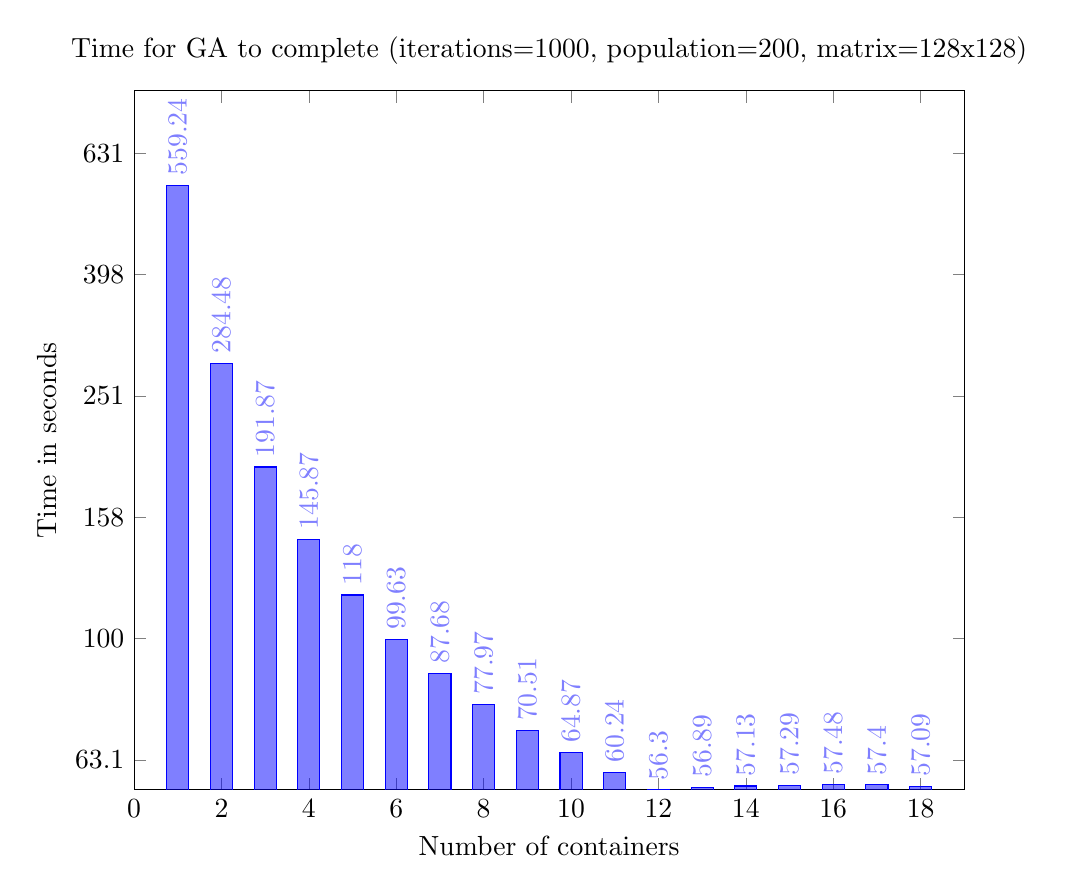
\begin{tikzpicture}[]
    \begin{semilogyaxis}[
	title={Time for GA to complete (iterations=1000, population=200, matrix=128x128)},
	xlabel={Number of containers},
	ylabel={Time in seconds},
	width=\linewidth,
	enlargelimits=false,
% 	nodes near coords,
	log ticks with fixed point,
	nodes near coords=\rotatebox{90}{\pgfmathprintnumber[]\value},
	visualization depends on=rawy \as \value,
	xmin=0,
	xmax=19,
	ymin=0,
	ymax=800
      ]
      \addplot[ybar, bar width=8pt, blue, fill, fill opacity=0.5]
      coordinates{(1,559.241803922) (2,284.478117647) (3,191.86994) (4,145.866961538) (5,117.99764) (6,99.62942) (7,87.68198) (8,77.97484) (9,70.50712) (10,64.87274) (11,60.23614) (12,56.29868) (13,56.88716) (14,57.1284) (15,57.29426) (16,57.4755490196) (17,57.4018) (18,57.08912)};
    \end{semilogyaxis}
  \end{tikzpicture}
  \caption{Find an optimal tile size for the tiled matrix multiplication. The x-axis shows the number of containers (workers), the y-axis shows the time it took to finish on a logarithmic scale. iterations=1000, population=200, matrix size=128x128}
  \label{plot:tiledmul_1000_200_128x128_log}
\end{figure}

\begin{table}
  \centering
  \begin{tabular}{l|r|r}
    & x & y \\ \hline
    min & 128 & 7 \\
    max & 128 & 126 \\
    mean & 128.0 & 19.0143646409 \\
    var & 0.0 & 113.070511889 \\
    stddev & 0.0 & 10.6334618958 \\
  \end{tabular}
  \caption{Results for tile sizes, iterations=1000, population=200, matrix size=128x128}
  \label{table:tiledmul_1000_200_128x128}
\end{table}


% \section{Population 50 matrix 256x256}
\begin{figure}[h]
  \centering
  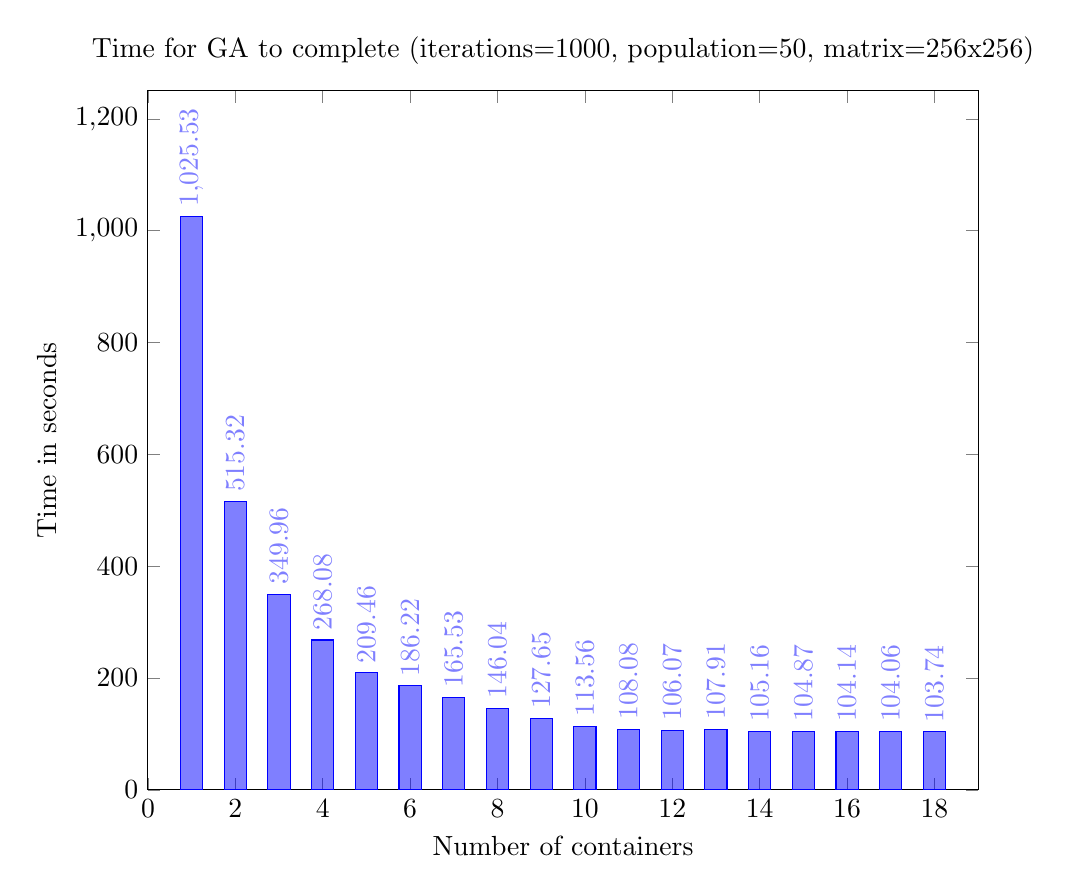
\begin{tikzpicture}[]
    \begin{axis}[
	title={Time for GA to complete (iterations=1000, population=50, matrix=256x256)},
	xlabel={Number of containers},
	ylabel={Time in seconds},
	width=\linewidth,
	enlargelimits=false,
	nodes near coords=\rotatebox{90}{\pgfmathprintnumber[]\value},
	visualization depends on=rawy \as \value,
	xmin=0,
	xmax=19,
	ymin=0,
	ymax=1250
      ]
      \addplot[ybar, bar width=8pt, blue, fill, fill opacity=0.5]
      coordinates{(1,1025.53004) (2,515.317313725) (3,349.96234) (4,268.08298) (5,209.458882353) (6,186.215529412) (7,165.52684) (8,146.03526) (9,127.64504) (10,113.56404) (11,108.08478) (12,106.07322) (13,107.9095) (14,105.15728) (15,104.8745) (16,104.14066) (17,104.0597) (18,103.7404)};
%       \addplot [red, no markers] coordinates {(0,0) (12,38.4)};
    \end{axis}
  \end{tikzpicture}
  \caption{Find an optimal tile size for the tiled matrix multiplication. The x-axis shows the number of containers (workers), the y-axis shows the time it took to finish. iterations=1000, population=50, matrix size=256x256}
\label{plot:tiledmul_1000_50_256x256}
\end{figure}

\begin{figure}[h]
  \centering
  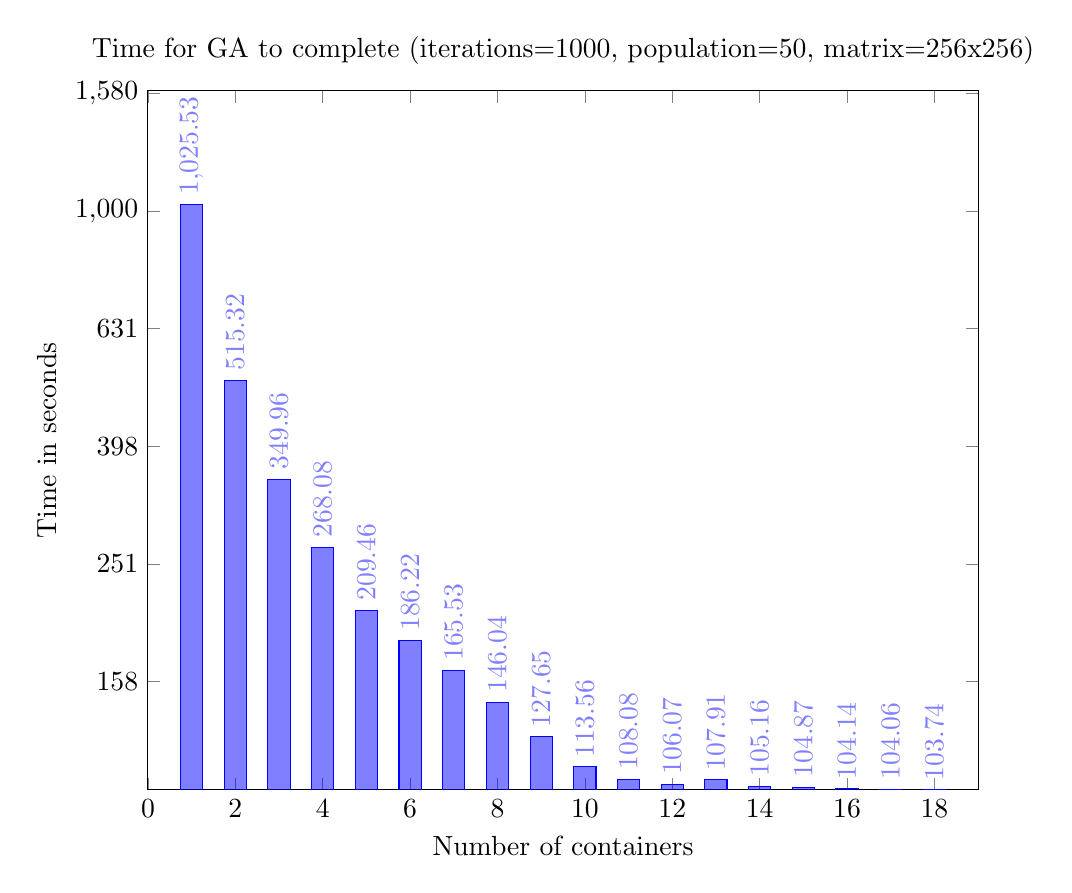
\begin{tikzpicture}[]
    \begin{semilogyaxis}[
	title={Time for GA to complete (iterations=1000, population=50, matrix=256x256)},
	xlabel={Number of containers},
	ylabel={Time in seconds},
	width=\linewidth,
	enlargelimits=false,
% 	nodes near coords,
	log ticks with fixed point,
	nodes near coords=\rotatebox{90}{\pgfmathprintnumber[]\value},
	visualization depends on=rawy \as \value,
	xmin=0,
	xmax=19,
	ymin=0,
	ymax=1600
      ]
      \addplot[ybar, bar width=8pt, blue, fill, fill opacity=0.5]
      coordinates{(1,1025.53004) (2,515.317313725) (3,349.96234) (4,268.08298) (5,209.458882353) (6,186.215529412) (7,165.52684) (8,146.03526) (9,127.64504) (10,113.56404) (11,108.08478) (12,106.07322) (13,107.9095) (14,105.15728) (15,104.8745) (16,104.14066) (17,104.0597) (18,103.7404)};
    \end{semilogyaxis}
  \end{tikzpicture}
  \caption{Find an optimal tile size for the tiled matrix multiplication. The x-axis shows the number of containers (workers), the y-axis shows the time it took to finish on a logarithmic scale. iterations=1000, population=50, matrix size=256x256}
  \label{plot:tiledmul_1000_50_256x256_log}
\end{figure}

\begin{table}
  \centering
  \begin{tabular}{l|r|r}
    & x & y \\ \hline
    min & 142 & 4 \\
    max & 256 & 256 \\
    mean & 254.686600221 & 25.1716500554 \\
    var & 116.328137168 & 2519.74573006 \\
    stddev & 10.7855522421 & 50.1970689389 \\
  \end{tabular}
  \caption{Results for tile sizes, iterations=1000, population=50, matrix size=256x256}
  \label{table:tiledmul_1000_50_256x256}
\end{table}

% \section{Population 100 matrix 256x256}
\begin{figure}[h]
  \centering
  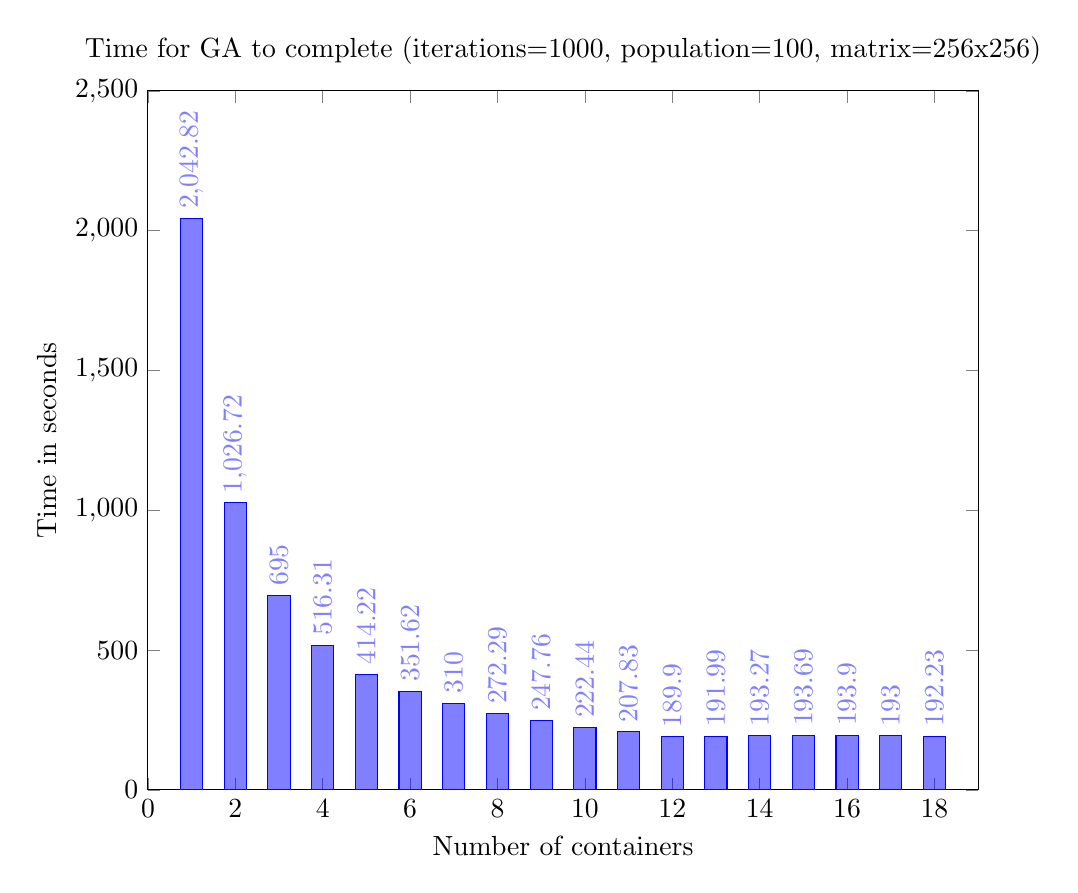
\begin{tikzpicture}[]
    \begin{axis}[
	title={Time for GA to complete (iterations=1000, population=100, matrix=256x256)},
	xlabel={Number of containers},
	ylabel={Time in seconds},
	width=\linewidth,
	enlargelimits=false,
	nodes near coords=\rotatebox{90}{\pgfmathprintnumber[]\value},
	visualization depends on=rawy \as \value,
	xmin=0,
	xmax=19,
	ymin=0,
	ymax=2500
      ]
      \addplot[ybar, bar width=8pt, blue, fill, fill opacity=0.5]
      coordinates{(1,2042.8174) (2,1026.7248) (3,694.9952) (4,516.314166667) (5,414.2218) (6,351.6154) (7,310.0028) (8,272.2884) (9,247.756) (10,222.435) (11,207.8292) (12,189.9014) (13,191.9934) (14,193.2658) (15,193.6938) (16,193.8992) (17,193.0012) (18,192.2272)};
%       \addplot [red, no markers] coordinates {(0,0) (12,38.4)};
    \end{axis}
  \end{tikzpicture}
  \caption{Find an optimal tile size for the tiled matrix multiplication. The x-axis shows the number of containers (workers), the y-axis shows the time it took to finish. iterations=1000, population=100, matrix size=256x256}
\label{plot:tiledmul_1000_100_256x256}
\end{figure}

\begin{figure}[h]
  \centering
  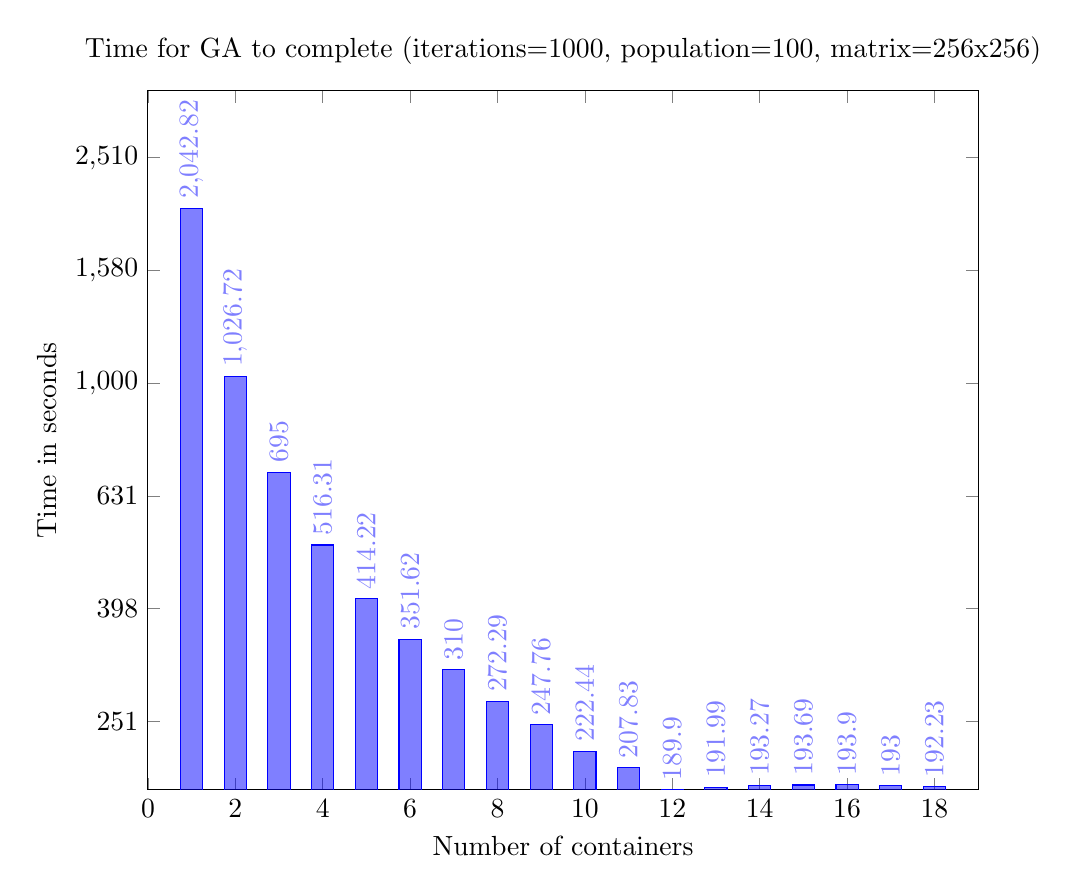
\begin{tikzpicture}[]
    \begin{semilogyaxis}[
	title={Time for GA to complete (iterations=1000, population=100, matrix=256x256)},
	xlabel={Number of containers},
	ylabel={Time in seconds},
	width=\linewidth,
	enlargelimits=false,
% 	nodes near coords,
	log ticks with fixed point,
	nodes near coords=\rotatebox{90}{\pgfmathprintnumber[]\value},
	visualization depends on=rawy \as \value,
	xmin=0,
	xmax=19,
	ymin=0,
	ymax=3300
      ]
      \addplot[ybar, bar width=8pt, blue, fill, fill opacity=0.5]
      coordinates{(1,2042.8174) (2,1026.7248) (3,694.9952) (4,516.314166667) (5,414.2218) (6,351.6154) (7,310.0028) (8,272.2884) (9,247.756) (10,222.435) (11,207.8292) (12,189.9014) (13,191.9934) (14,193.2658) (15,193.6938) (16,193.8992) (17,193.0012) (18,192.2272)};
    \end{semilogyaxis}
  \end{tikzpicture}
  \caption{Find an optimal tile size for the tiled matrix multiplication. The x-axis shows the number of containers (workers), the y-axis shows the time it took to finish on a logarithmic scale. iterations=1000, population=100, matrix size=256x256}
  \label{plot:tiledmul_1000_100_256x256_log}
\end{figure}

\begin{table}
  \centering
  \begin{tabular}{l|r|r}
    & x & y \\ \hline
    min & 256 & 6 \\
    max & 256 & 245 \\
    mean & 256.0 & 20.3956043956 \\
    var & 0.0 & 2163.71162903 \\
    stddev & 0.0 & 46.5157137861 \\
  \end{tabular}
  \caption{Results for tile sizes, iterations=1000, population=100, matrix size=256x256}
  \label{table:tiledmul_1000_100_256x256}
\end{table}

% \section{Population 200 matrix 256x256}
\begin{figure}[h]
  \centering
  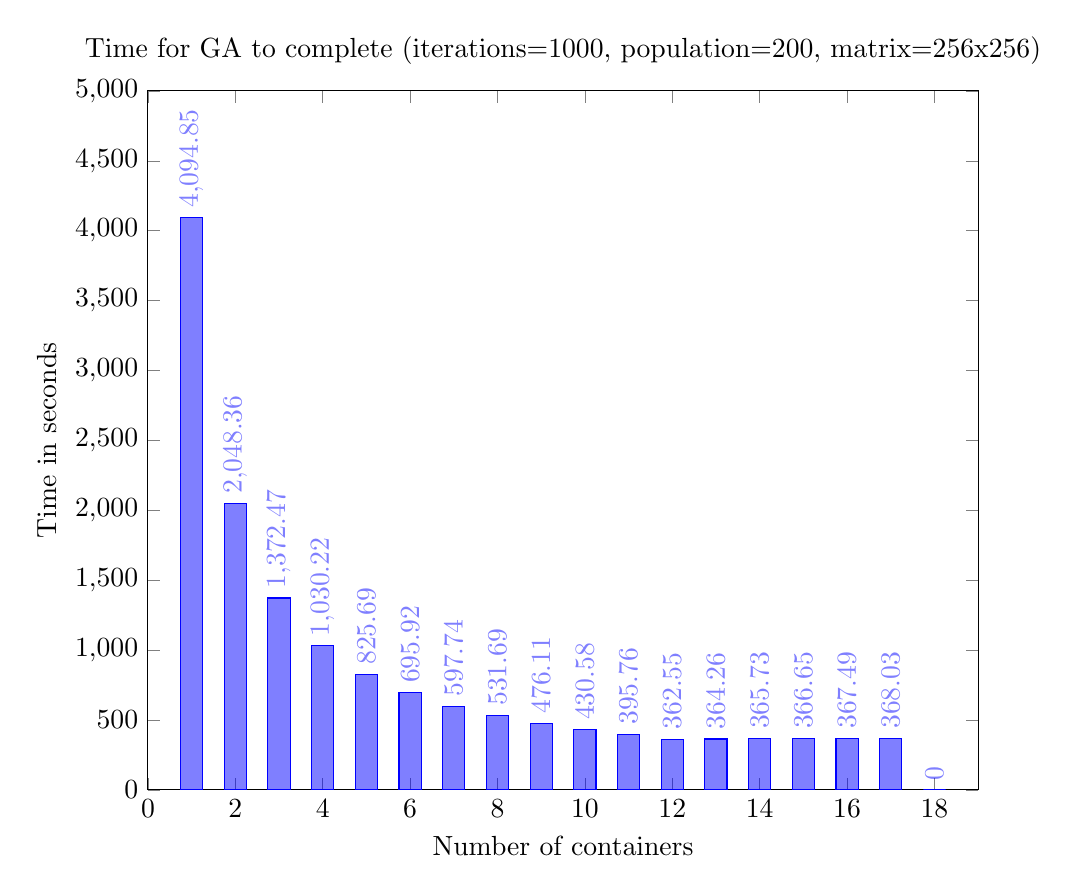
\begin{tikzpicture}[]
    \begin{axis}[
	title={Time for GA to complete (iterations=1000, population=200, matrix=256x256)},
	xlabel={Number of containers},
	ylabel={Time in seconds},
	width=\linewidth,
	enlargelimits=false,
	nodes near coords=\rotatebox{90}{\pgfmathprintnumber[]\value},
	visualization depends on=rawy \as \value,
	xmin=0,
	xmax=19,
	ymin=0,
	ymax=5000
      ]
      \addplot[ybar, bar width=8pt, blue, fill, fill opacity=0.5]
      coordinates{(1,4094.8474) (2,2048.359) (3,1372.4704) (4,1030.2228) (5,825.6862) (6,695.9234) (7,597.7398) (8,531.6904) (9,476.109) (10,430.5758) (11,395.7612) (12,362.5518) (13,364.2562) (14,365.7298) (15,366.645) (16,367.4866) (17,368.0268) (18,0)};
%       \addplot [red, no markers] coordinates {(0,0) (12,38.4)};
    \end{axis}
  \end{tikzpicture}
  \caption{Find an optimal tile size for the tiled matrix multiplication. The x-axis shows the number of containers (workers), the y-axis shows the time it took to finish. iterations=1000, population=200, matrix size=256x256}
\label{plot:tiledmul_1000_200_256x256}
\end{figure}

\begin{figure}[h]
  \centering
  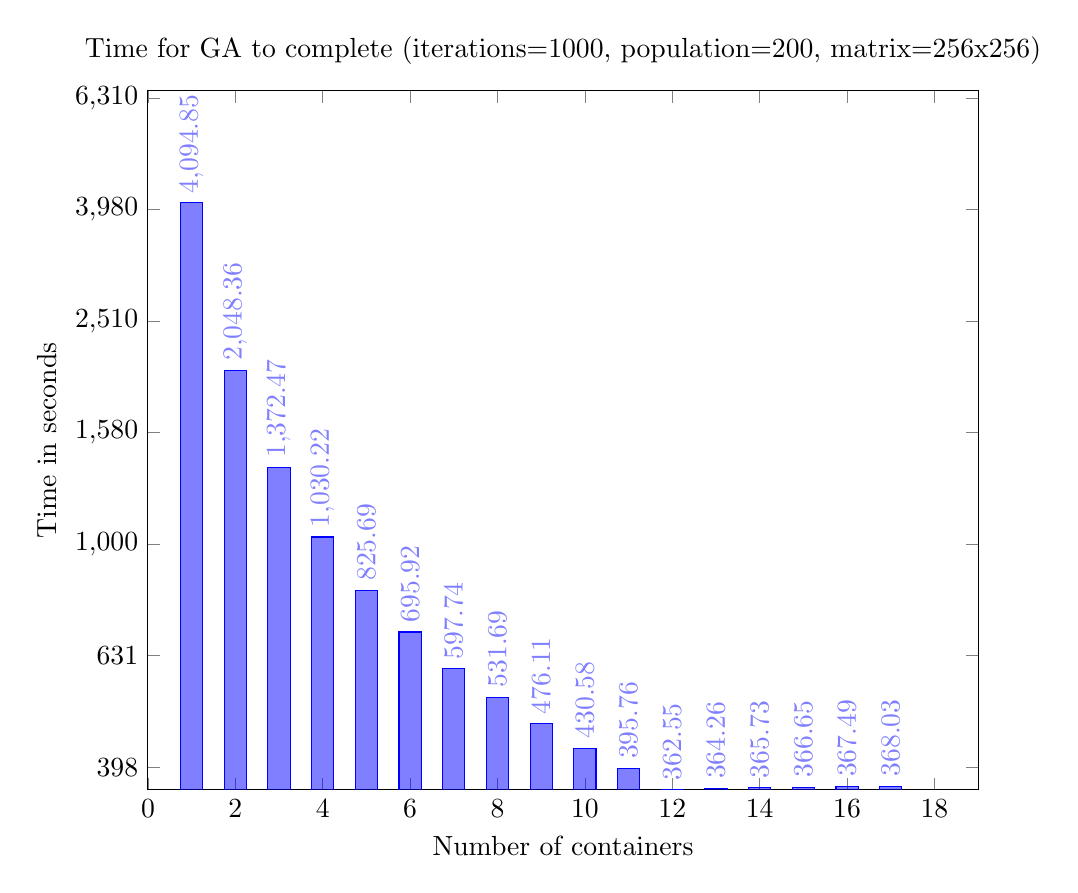
\begin{tikzpicture}[]
    \begin{semilogyaxis}[
	title={Time for GA to complete (iterations=1000, population=200, matrix=256x256)},
	xlabel={Number of containers},
	ylabel={Time in seconds},
	width=\linewidth,
	enlargelimits=false,
% 	nodes near coords,
	log ticks with fixed point,
	nodes near coords=\rotatebox{90}{\pgfmathprintnumber[]\value},
	visualization depends on=rawy \as \value,
	xmin=0,
	xmax=19,
	ymin=0,
	ymax=6500
      ]
      \addplot[ybar, bar width=8pt, blue, fill, fill opacity=0.5]
      coordinates{(1,4094.8474) (2,2048.359) (3,1372.4704) (4,1030.2228) (5,825.6862) (6,695.9234) (7,597.7398) (8,531.6904) (9,476.109) (10,430.5758) (11,395.7612) (12,362.5518) (13,364.2562) (14,365.7298) (15,366.645) (16,367.4866) (17,368.0268) (18,0)};
    \end{semilogyaxis}
  \end{tikzpicture}
  \caption{Find an optimal tile size for the tiled matrix multiplication. The x-axis shows the number of containers (workers), the y-axis shows the time it took to finish on a logarithmic scale. iterations=1000, population=200, matrix size=256x256}
  \label{plot:tiledmul_1000_200_256x256_log}
\end{figure}

\begin{table}
  \centering
  \begin{tabular}{l|r|r}
    & x & y \\ \hline
    min & 256 & 6 \\
    max & 256 & 251 \\
    mean & 256.0 & 16.8823529412 \\
    var & 0.0 & 1495.68027682 \\
    stddev & 0.0 & 38.6740258677 \\
  \end{tabular}
  \caption{Results for tile sizes, iterations=1000, population=200, matrix size=256x256}
  \label{table:tiledmul_1000_200_256x256}
\end{table}

% \section{Population 50 matrix 512x512}
\clearpage
\begin{figure}[h]
  \centering
  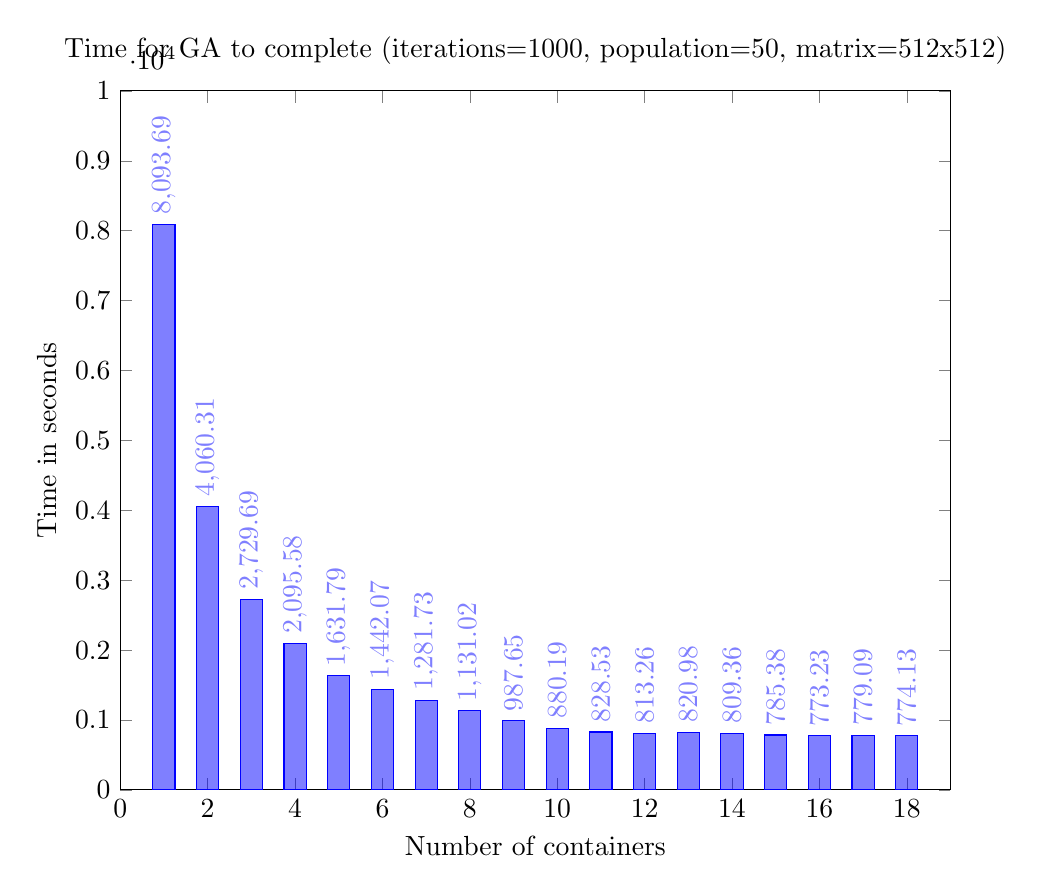
\begin{tikzpicture}[]
    \begin{axis}[
	title={Time for GA to complete (iterations=1000, population=50, matrix=512x512)},
	xlabel={Number of containers},
	ylabel={Time in seconds},
	width=\linewidth,
	enlargelimits=false,
	nodes near coords=\rotatebox{90}{\pgfmathprintnumber[]\value},
	visualization depends on=rawy \as \value,
	xmin=0,
	xmax=19,
	ymin=0,
	ymax=10000
      ]
      \addplot[ybar, bar width=8pt, blue, fill, fill opacity=0.5]
      coordinates{(1,8093.694) (2,4060.3118) (3,2729.6922) (4,2095.5812) (5,1631.7902) (6,1442.0658) (7,1281.734) (8,1131.0154) (9,987.65) (10,880.191) (11,828.5316) (12,813.263) (13,820.9774) (14,809.3636) (15,785.3828) (16,773.2344) (17,779.0904) (18,774.1268)};
%       \addplot [red, no markers] coordinates {(0,0) (12,38.4)};
    \end{axis}
  \end{tikzpicture}
  \caption{Find an optimal tile size for the tiled matrix multiplication. The x-axis shows the number of containers (workers), the y-axis shows the time it took to finish. iterations=1000, population=50, matrix size=512x512}
\label{plot:tiledmul_1000_50_512x512}
\end{figure}

\begin{figure}[h]
  \centering
  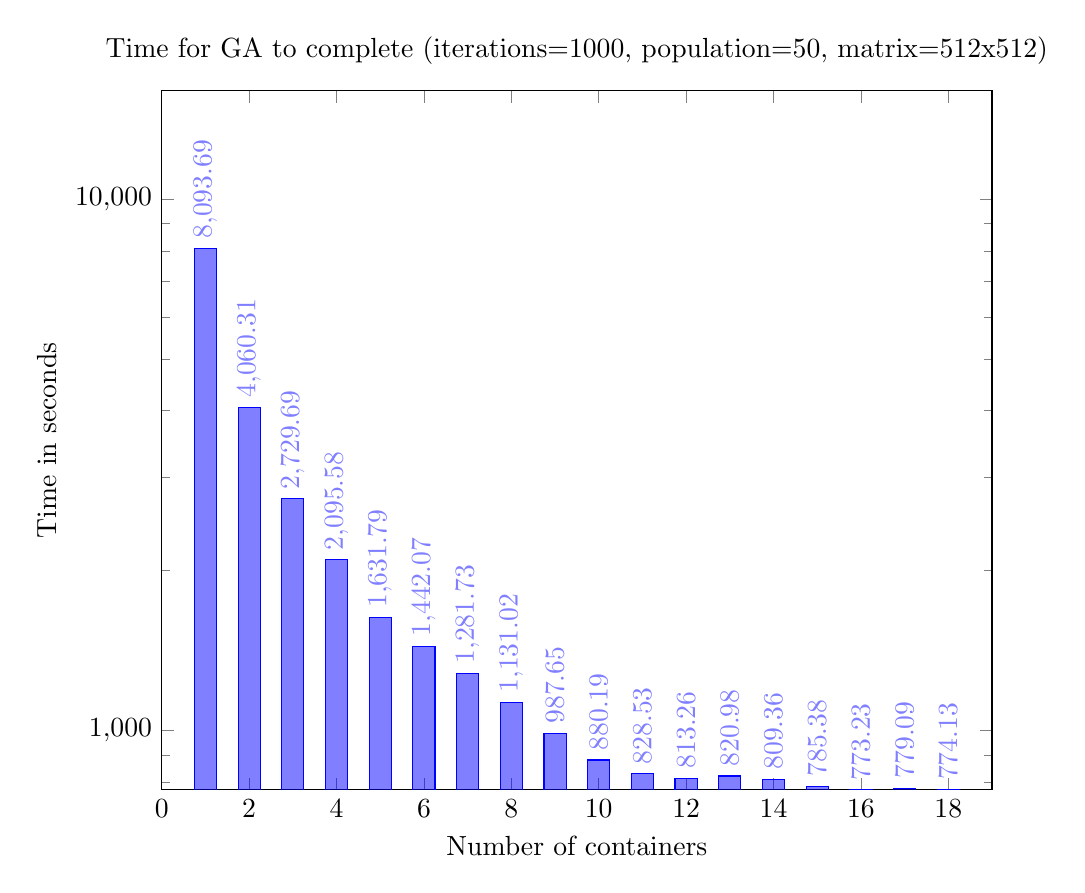
\begin{tikzpicture}[]
    \begin{semilogyaxis}[
	title={Time for GA to complete (iterations=1000, population=50, matrix=512x512)},
	xlabel={Number of containers},
	ylabel={Time in seconds},
	width=\linewidth,
	enlargelimits=false,
% 	nodes near coords,
	log ticks with fixed point,
	nodes near coords=\rotatebox{90}{\pgfmathprintnumber[]\value},
	visualization depends on=rawy \as \value,
	xmin=0,
	xmax=19,
	ymin=0,
	ymax=16000
      ]
      \addplot[ybar, bar width=8pt, blue, fill, fill opacity=0.5]
      coordinates{(1,8093.694) (2,4060.3118) (3,2729.6922) (4,2095.5812) (5,1631.7902) (6,1442.0658) (7,1281.734) (8,1131.0154) (9,987.65) (10,880.191) (11,828.5316) (12,813.263) (13,820.9774) (14,809.3636) (15,785.3828) (16,773.2344) (17,779.0904) (18,774.1268)};
    \end{semilogyaxis}
  \end{tikzpicture}
  \caption{Find an optimal tile size for the tiled matrix multiplication. The x-axis shows the number of containers (workers), the y-axis shows the time it took to finish on a logarithmic scale. iterations=1000, population=50, matrix size=512x512}
  \label{plot:tiledmul_1000_50_512x512_log}
\end{figure}

\begin{table}
  \centering
  \begin{tabular}{l|r|r}
    & x & y \\ \hline
    min & 258 & 3 \\
    max & 512 & 512 \\
    mean & 479.522222222 & 115.355555556 \\
    var & 6292.11617284 & 22195.3846914 \\
    stddev & 79.322860342 & 148.981155491 \\
  \end{tabular}
  \caption{Results for tile sizes, iterations=1000, population=50, matrix=512x512}
  \label{table:tiledmul_1000_50_512x512}
\end{table}
  
\end{document}
